\documentclass[11pt]{article}
\usepackage{graphicx}


\begin{document}
\title{Driven Damped Pendulum and Chaos}
\author{Colt Bradley}
\date{}
\maketitle

\section{Part 1}

For the first part, we analyze systems with the initial condition $\theta_i = 0 $ for the cases $\gamma = 0.6, 1.073, 1.077 $. We run our RK4 code with 128000 time steps, which from the previous exercise we know is accurate to approximately 8 decimal places. 

$\gamma$ determines how strong the driving force is. With weaker driving force, we should see that the periodic motion should stabilize sooner. With three graphs on the left, we see that the first stabilizes sooner than any of the other graphs. When it stabilizes we can determine the period, which seems to to be $2 \pi$ as we would expect. Before it stabilizes, the motion is chaotic.

For the graphs in phase space, a non-chaotic periodic system would look like a circle. The further perturbed from a circle the phase space trajectory appears the more chaotic the system is.  

\begin{figure}[ht]
\begin{tabular}{cc}
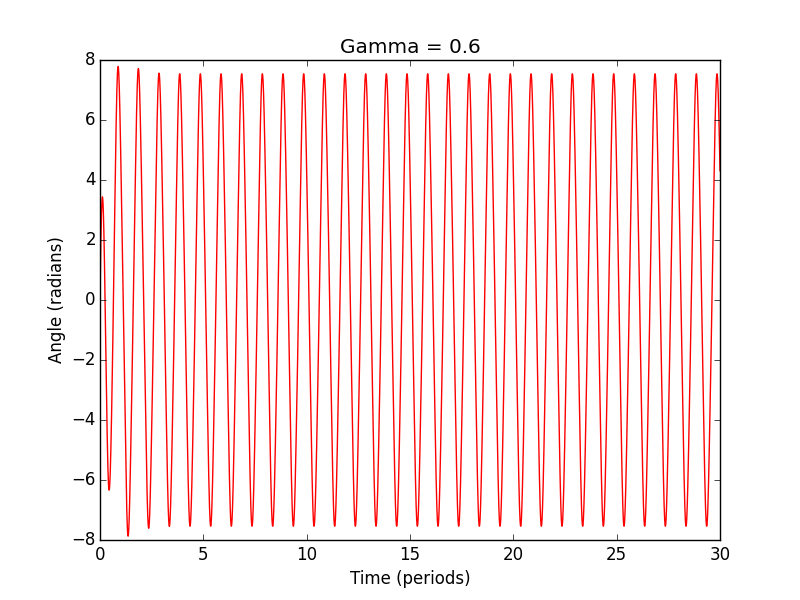
\includegraphics[scale=.4]{g6theta.png}&

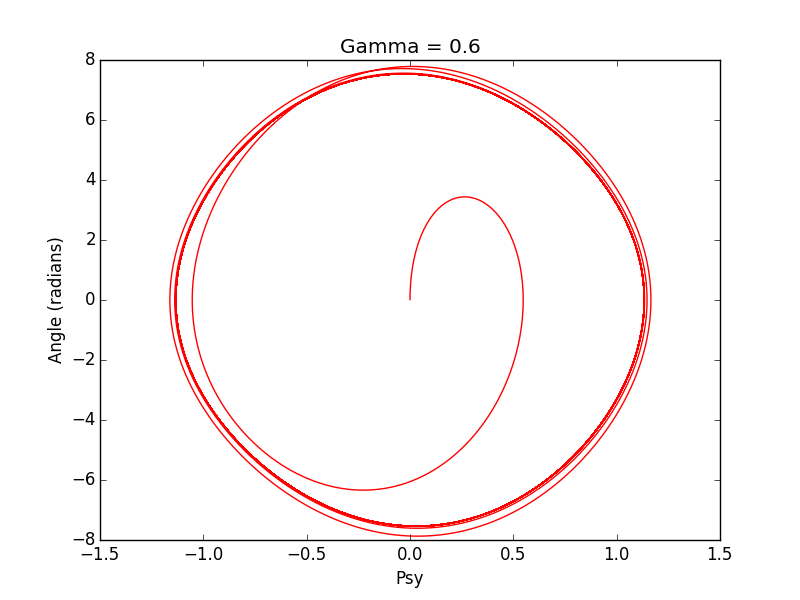
\includegraphics[scale=.4]{g6psy.png} \\
\multicolumn{2}{c}{(a) $\gamma = 0.6 $} \\[6pt]

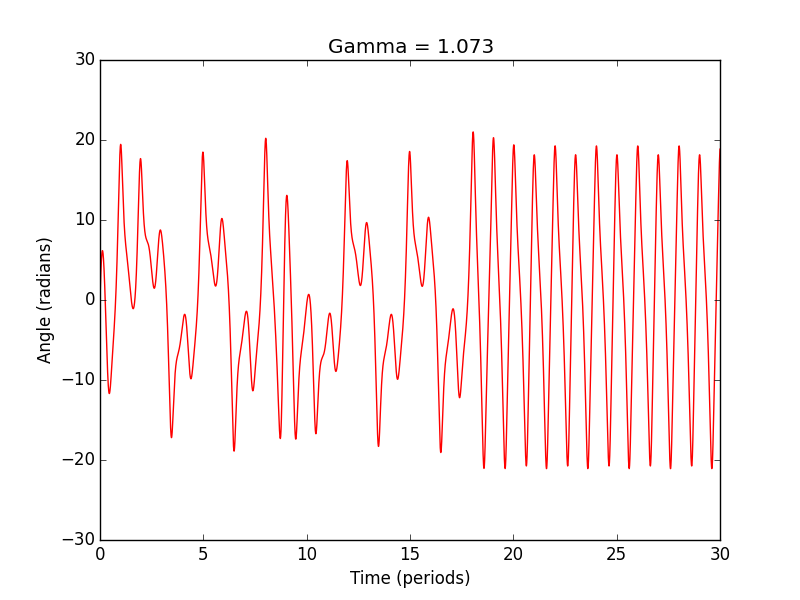
\includegraphics[scale=.4]{g073theta.png}&

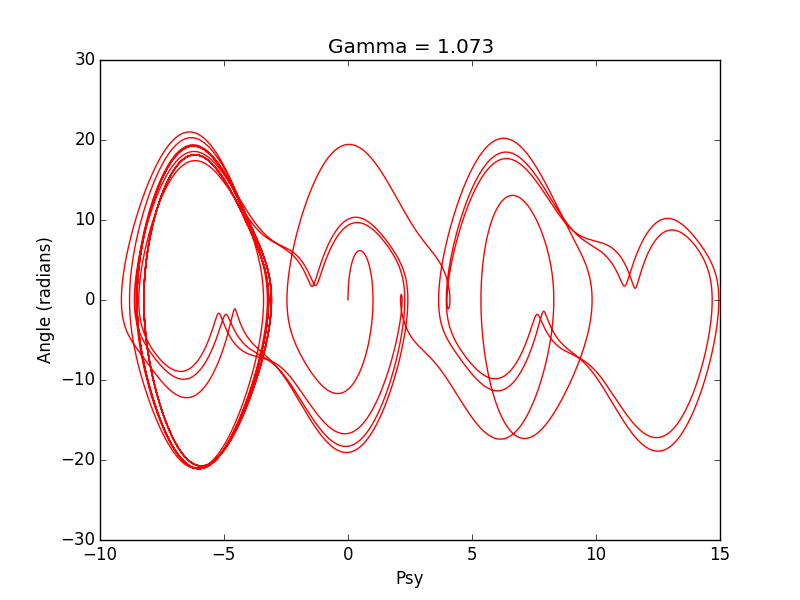
\includegraphics[scale=.4]{g073psy.png}\\
\multicolumn{2}{c}{(b) $\gamma = 1.073 $} \\[6pt]

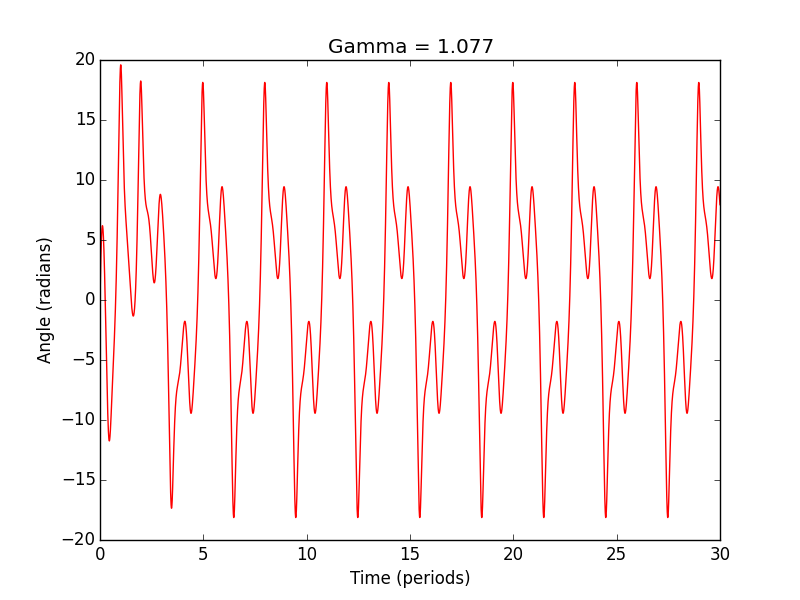
\includegraphics[scale=.4]{g077theta.png}&

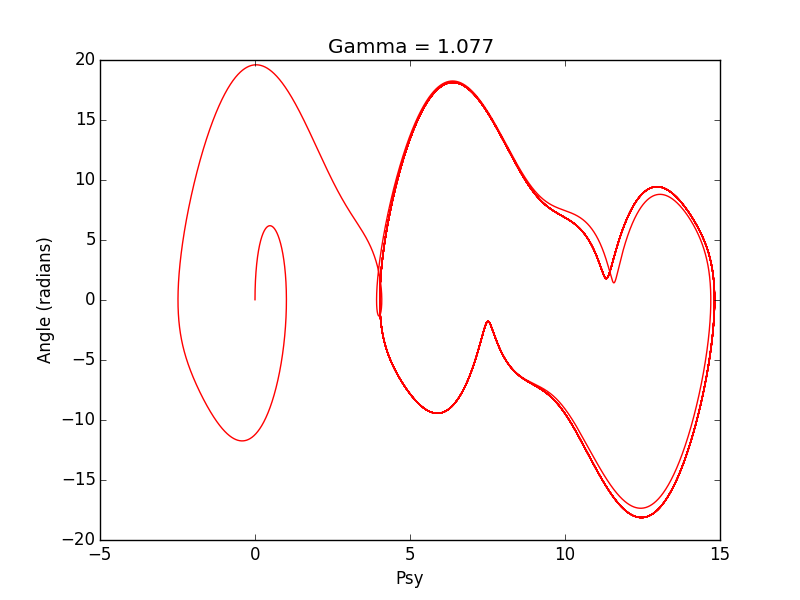
\includegraphics[scale=.4]{g077psy.png}\\
\multicolumn{2}{c}{(c) $\gamma = 1.077 $} \\[6pt]
\end{tabular}
\caption{Various plots for $\theta_i = 0 $}

\end{figure}

\section{Part 2}

Now, we analyze systems with the initial condition $\theta_i = - \pi /2 $ for the cases $\gamma = 1.08, 1.1, 1.2, 1.25 $. 

As before, once the system stabilizes then the period is $2 \pi$, as before. For the phase space plots, we see similar trajectories to before, but the final trajectory seems considerably more chaotic. 

\begin{figure}[ht]
\begin{tabular}{cc}
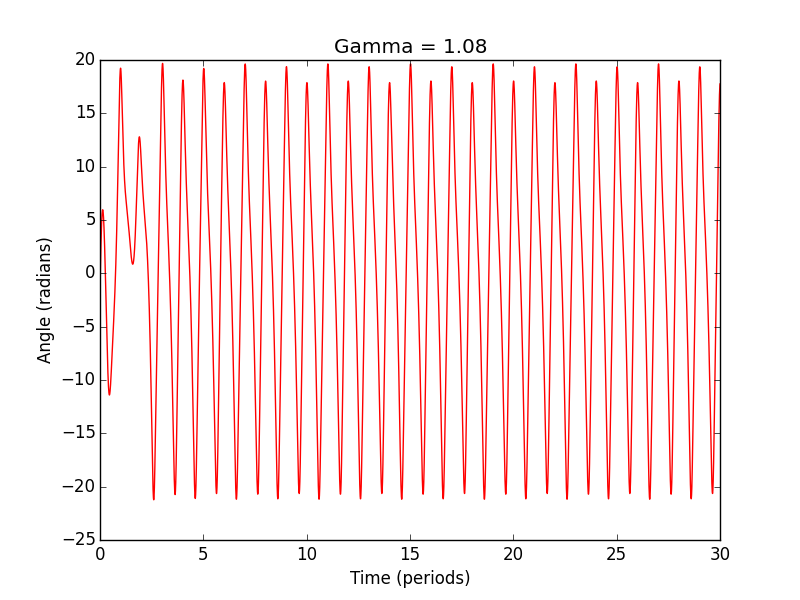
\includegraphics[scale=.3]{g08theta.png}&

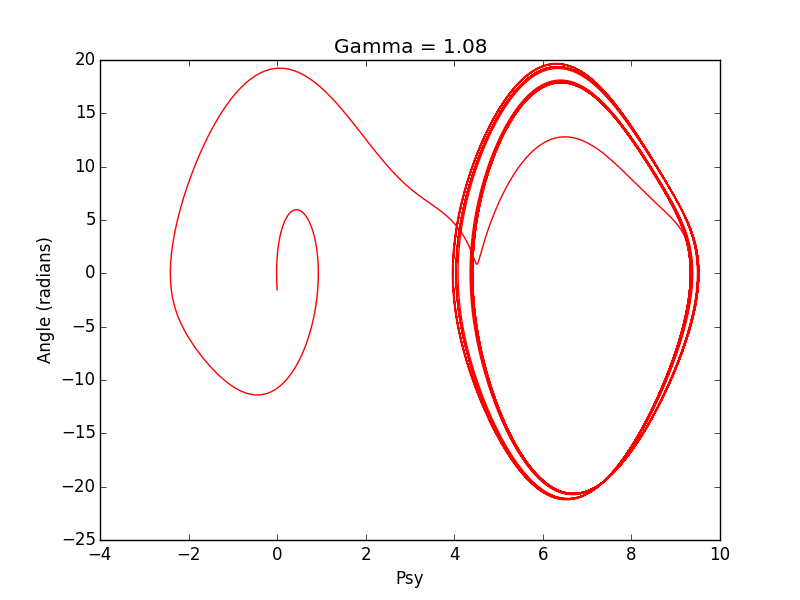
\includegraphics[scale=.3]{g08psy.png} \\
\multicolumn{2}{c}{(a) $\gamma = 1.08 $} \\[6pt]

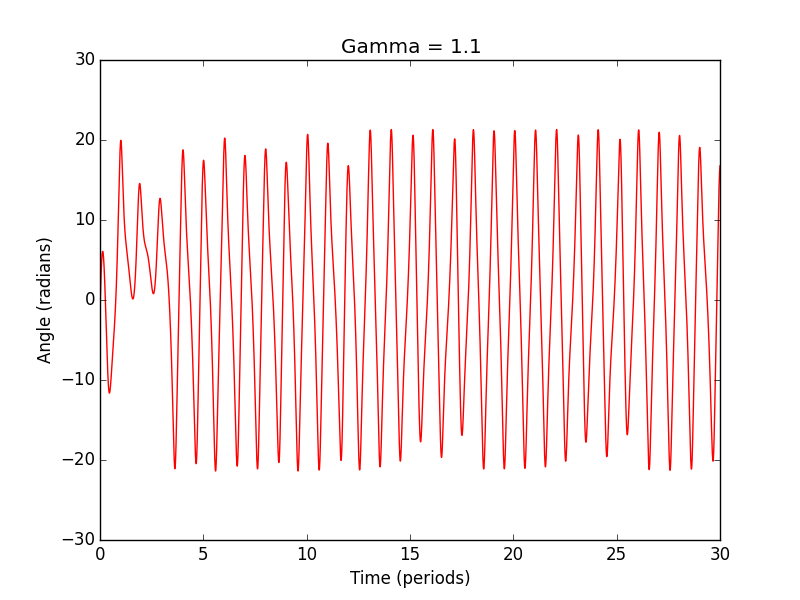
\includegraphics[scale=.3]{g1theta.png}&

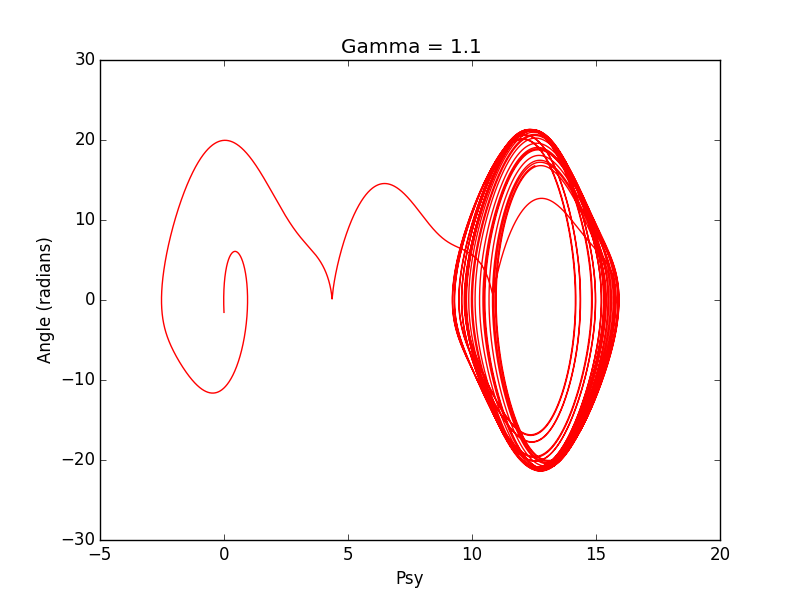
\includegraphics[scale=.3]{g1psy.png}\\
\multicolumn{2}{c}{(b) $\gamma = 1.1 $} \\[6pt]

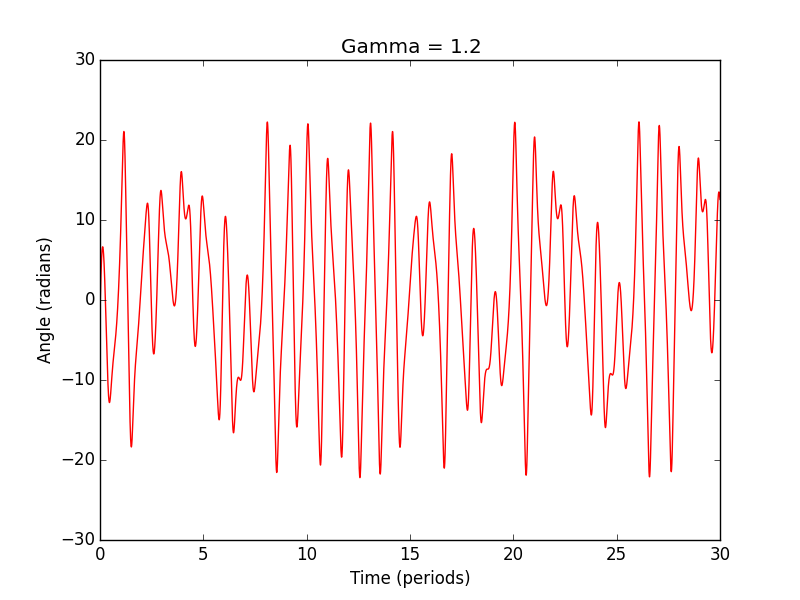
\includegraphics[scale=.3]{g2theta.png}&

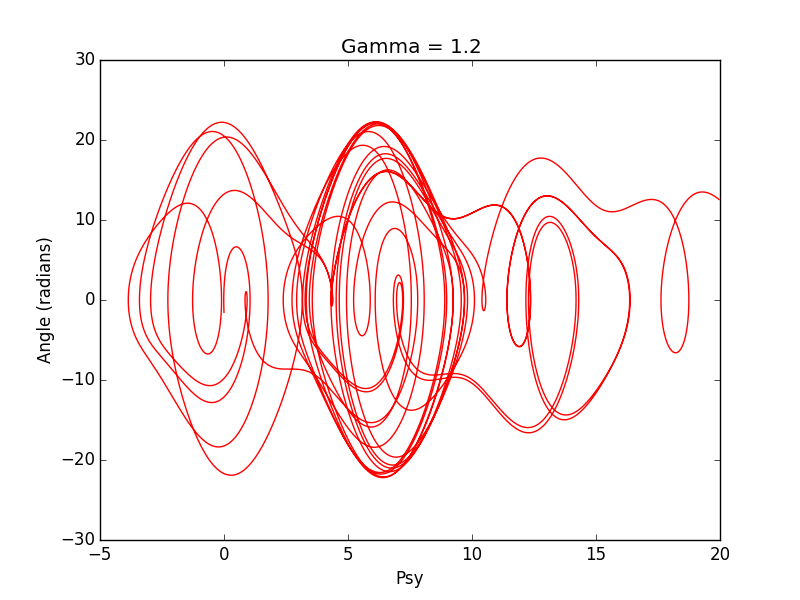
\includegraphics[scale=.3]{g2psy.png}\\
\multicolumn{2}{c}{(c) $\gamma = 1.2 $} \\[6pt]\\

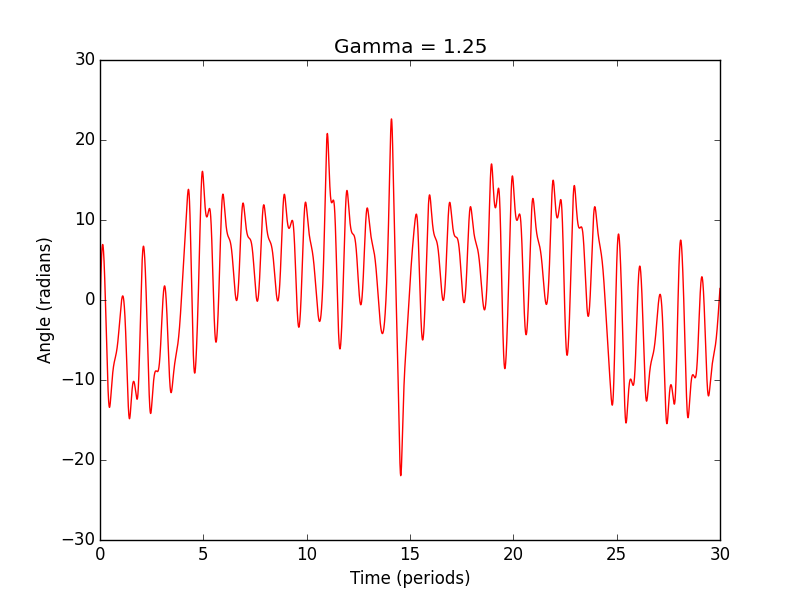
\includegraphics[scale=.3]{g25theta.png}&

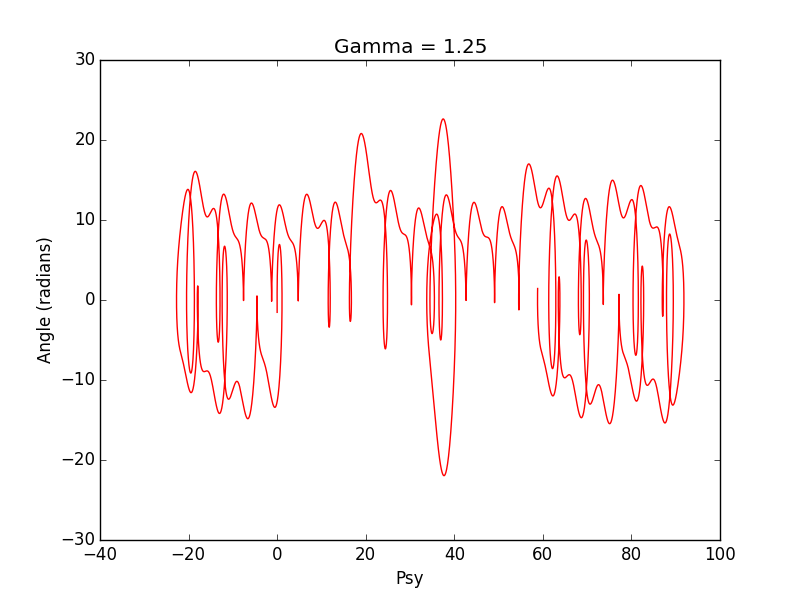
\includegraphics[scale=.3]{g25psy.png}\\
\multicolumn{2}{c}{(d) $\gamma = 1.25 $} \\[6pt]
\end{tabular}
\caption{Various plots for $\theta_i = - \pi /2 $}

\end{figure}

\section{Comparing Chaotic and non-chaotic systems}

We'd like to see the difference between chaotic and non-chaotic systems. We can preform this by solving the equation with slightly different initial conditions ($\theta_i = - \pi /2 $ and $\theta_i = - \pi /2 +0.0001 $). For one system, we set $\gamma = 1.25$ which creates a chaotic system. The next, we set $\gamma = 0$. We can graph the difference in the angles between these two systems. For a non-chaotic system the difference should be minimal, but for a chaotic system the difference can be a lot. 

In the chaotic system, the difference in angle doesn't follow any specific pattern. In the non-chaotic system, the difference decreases exponentially.  

\begin{figure}
\begin{tabular}{cc}
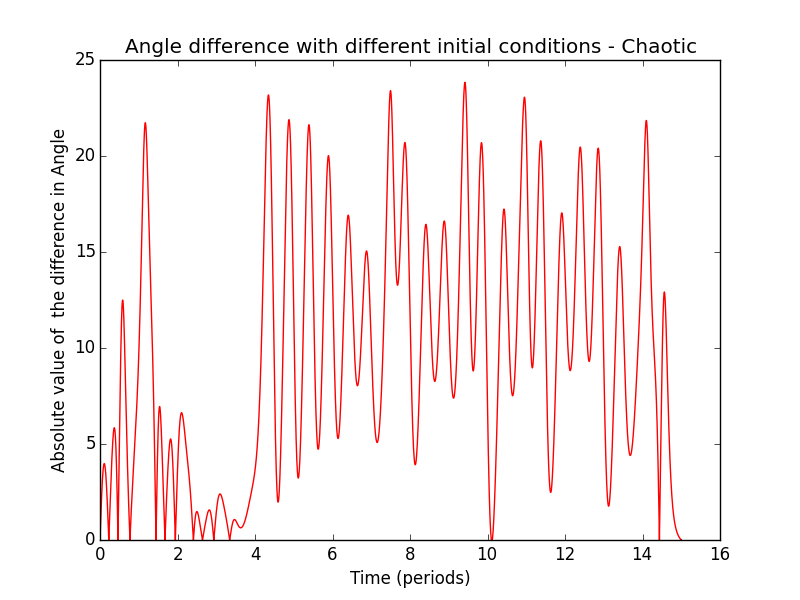
\includegraphics[scale=.3]{deltathetachaos.png}&

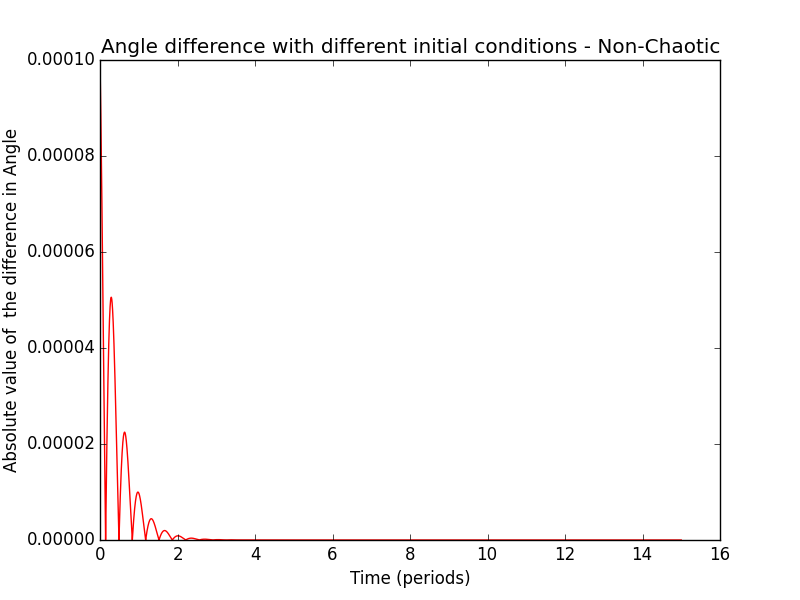
\includegraphics[scale=.3]{deltathetanochaos.png}\\
 $\gamma = 1.25 $ & $\gamma = 0 $ \\[6pt]
\end{tabular}
\caption{Comparison of Chaotic vs. Non-chaotic systems}
\end{figure}

\section{Code}

\begin{verbatim}
#Colt Bradley
#Lesson 18
#4.5.16

#import essential modules
import numpy as n
import pylab as p

def f(u,v,t):
    g = 1.25
    w = n.pi*2
    w0 = 1.5*w
    b = w0/4.
    return -w0**2*n.sin(u)-2*b*v+g*w0**2*n.cos(w*t)
    
#Initial Values and Setup    
time = []
N1 = []
N2 = []



t=n.linspace(0,15,128000)
dt = t[1]-t[0]
u = -n.pi/2
v = 0.
g = 1.25
w = n.pi*2
w0 = 1.5*w
b = w0/4.
U1 = []
U2 = []
V1 = []
V2 = []
for i in range (0,len(t)-1):
    ti = t[i]
    th = ti +dt/2.
    tf = t[i+1]
    time.append(ti)
    
    va = v +u*dt/2.
    ua = u +f(v,u,ti)*dt/2.
    vb = v +ua*dt/2.
    ub = u +f(va,ua,th)*dt/2.
    vc = v +ub*dt
    uc = u +f(vb,ub,th)*dt
    vd = v +uc*dt
    ud = u +f(vc,uc,tf)*dt
     
    v = (va+2*vb+vc+(vd/2.))/3-v/2
    u = (ua+2*ub+uc+(ud/2.))/3-u/2
        
    V1.append(v)
    U1.append(u)
N1.append(V1[-1])

u = -n.pi/2+.0001
for i in range (0,len(t)-1):
    ti = t[i]
    th = ti +dt/2.
    tf = t[i+1]
    
    va = v +u*dt/2.
    ua = u +f(v,u,ti)*dt/2.
    vb = v +ua*dt/2.
    ub = u +f(va,ua,th)*dt/2.
    vc = v +ub*dt
    uc = u +f(vb,ub,th)*dt
    vd = v +uc*dt
    ud = u +f(vc,uc,tf)*dt
     
    v = (va+2*vb+vc+(vd/2.))/3-v/2
    u = (ua+2*ub+uc+(ud/2.))/3-u/2
        
    V2.append(v)
    U2.append(u)
N2.append(V2[-1])

delta = n.zeros(len(U1))

for k in range(len(U1)):
    delta[k] = abs(U1[k]-U2[k])

p.close()
p.plot(time,delta,"r")
p.title("Angle difference with different initial conditions - Chaotic")
p.xlabel("Time (periods)")
p.ylabel("Absolute value of  the difference in Angle")
p.savefig("deltathetachaos.png")
p.show()
\end{verbatim}

\end{document}